% Options for packages loaded elsewhere
\PassOptionsToPackage{unicode}{hyperref}
\PassOptionsToPackage{hyphens}{url}
%
\documentclass[
  12pt,
]{article}
\usepackage{amsmath,amssymb}
\usepackage{lmodern}
\usepackage{ifxetex,ifluatex}
\ifnum 0\ifxetex 1\fi\ifluatex 1\fi=0 % if pdftex
  \usepackage[T1]{fontenc}
  \usepackage[utf8]{inputenc}
  \usepackage{textcomp} % provide euro and other symbols
\else % if luatex or xetex
  \usepackage{unicode-math}
  \defaultfontfeatures{Scale=MatchLowercase}
  \defaultfontfeatures[\rmfamily]{Ligatures=TeX,Scale=1}
\fi
% Use upquote if available, for straight quotes in verbatim environments
\IfFileExists{upquote.sty}{\usepackage{upquote}}{}
\IfFileExists{microtype.sty}{% use microtype if available
  \usepackage[]{microtype}
  \UseMicrotypeSet[protrusion]{basicmath} % disable protrusion for tt fonts
}{}
\makeatletter
\@ifundefined{KOMAClassName}{% if non-KOMA class
  \IfFileExists{parskip.sty}{%
    \usepackage{parskip}
  }{% else
    \setlength{\parindent}{0pt}
    \setlength{\parskip}{6pt plus 2pt minus 1pt}}
}{% if KOMA class
  \KOMAoptions{parskip=half}}
\makeatother
\usepackage{xcolor}
\IfFileExists{xurl.sty}{\usepackage{xurl}}{} % add URL line breaks if available
\IfFileExists{bookmark.sty}{\usepackage{bookmark}}{\usepackage{hyperref}}
\hypersetup{
  pdftitle={Stand Up Fight Back},
  pdfauthor={Kevin Morris; Kelsey Shoub},
  hidelinks,
  pdfcreator={LaTeX via pandoc}}
\urlstyle{same} % disable monospaced font for URLs
\usepackage[margin=1in]{geometry}
\usepackage{longtable,booktabs,array}
\usepackage{calc} % for calculating minipage widths
% Correct order of tables after \paragraph or \subparagraph
\usepackage{etoolbox}
\makeatletter
\patchcmd\longtable{\par}{\if@noskipsec\mbox{}\fi\par}{}{}
\makeatother
% Allow footnotes in longtable head/foot
\IfFileExists{footnotehyper.sty}{\usepackage{footnotehyper}}{\usepackage{footnote}}
\makesavenoteenv{longtable}
\usepackage{graphicx}
\makeatletter
\def\maxwidth{\ifdim\Gin@nat@width>\linewidth\linewidth\else\Gin@nat@width\fi}
\def\maxheight{\ifdim\Gin@nat@height>\textheight\textheight\else\Gin@nat@height\fi}
\makeatother
% Scale images if necessary, so that they will not overflow the page
% margins by default, and it is still possible to overwrite the defaults
% using explicit options in \includegraphics[width, height, ...]{}
\setkeys{Gin}{width=\maxwidth,height=\maxheight,keepaspectratio}
% Set default figure placement to htbp
\makeatletter
\def\fps@figure{htbp}
\makeatother
\setlength{\emergencystretch}{3em} % prevent overfull lines
\providecommand{\tightlist}{%
  \setlength{\itemsep}{0pt}\setlength{\parskip}{0pt}}
\setcounter{secnumdepth}{5}
\usepackage{rotating}
\usepackage{setspace}
\usepackage{booktabs}
\usepackage{longtable}
\usepackage{array}
\usepackage{multirow}
\usepackage{wrapfig}
\usepackage{float}
\usepackage{colortbl}
\usepackage{pdflscape}
\usepackage{tabu}
\usepackage{threeparttable}
\usepackage{threeparttablex}
\usepackage[normalem]{ulem}
\usepackage{makecell}
\usepackage{xcolor}
\ifluatex
  \usepackage{selnolig}  % disable illegal ligatures
\fi

\title{Stand Up Fight Back\thanks{Thanks.}}
\usepackage{etoolbox}
\makeatletter
\providecommand{\subtitle}[1]{% add subtitle to \maketitle
  \apptocmd{\@title}{\par {\large #1 \par}}{}{}
}
\makeatother
\subtitle{How Police Killings Can Mobilize Local Communities}
\author{Kevin Morris\footnote{Brennan Center for Justice, Researcher (\href{mailto:kevin.morris@nyu.edu}{\nolinkurl{kevin.morris@nyu.edu}})} \and Kelsey Shoub\footnote{University of South Carolina, Assistant Professor (\href{mailto:kshoub@mailbox.sc.edu}{\nolinkurl{kshoub@mailbox.sc.edu}})}}
\date{April 22, 2022}

\begin{document}
\maketitle
\begin{abstract}
TKTKTKTK
\end{abstract}

\pagenumbering{gobble}
\pagebreak
\doublespacing

\pagenumbering{arabic}

\begin{figure}[h]

{\centering 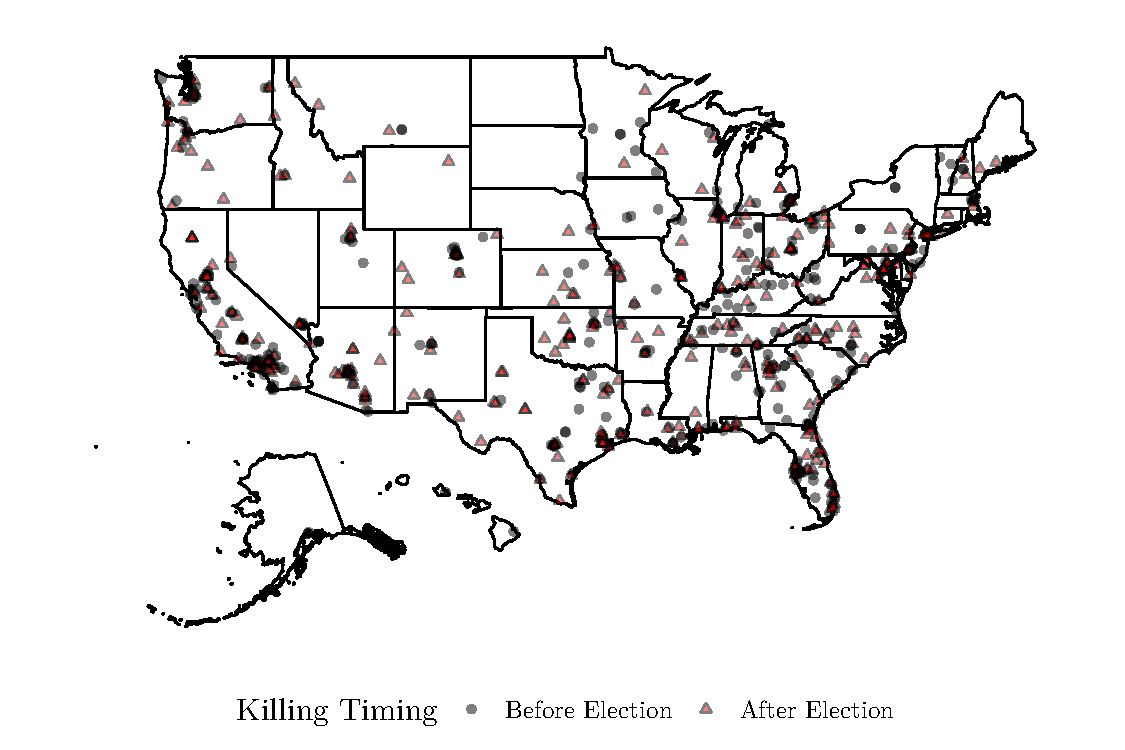
\includegraphics{shoot_to_files/figure-latex/map-1} 

}

\caption{\label{fig:map}Police Killing within 2 Months of Election, 2016 and 2020}\label{fig:map}
\end{figure}

\begin{figure}[h]

{\centering 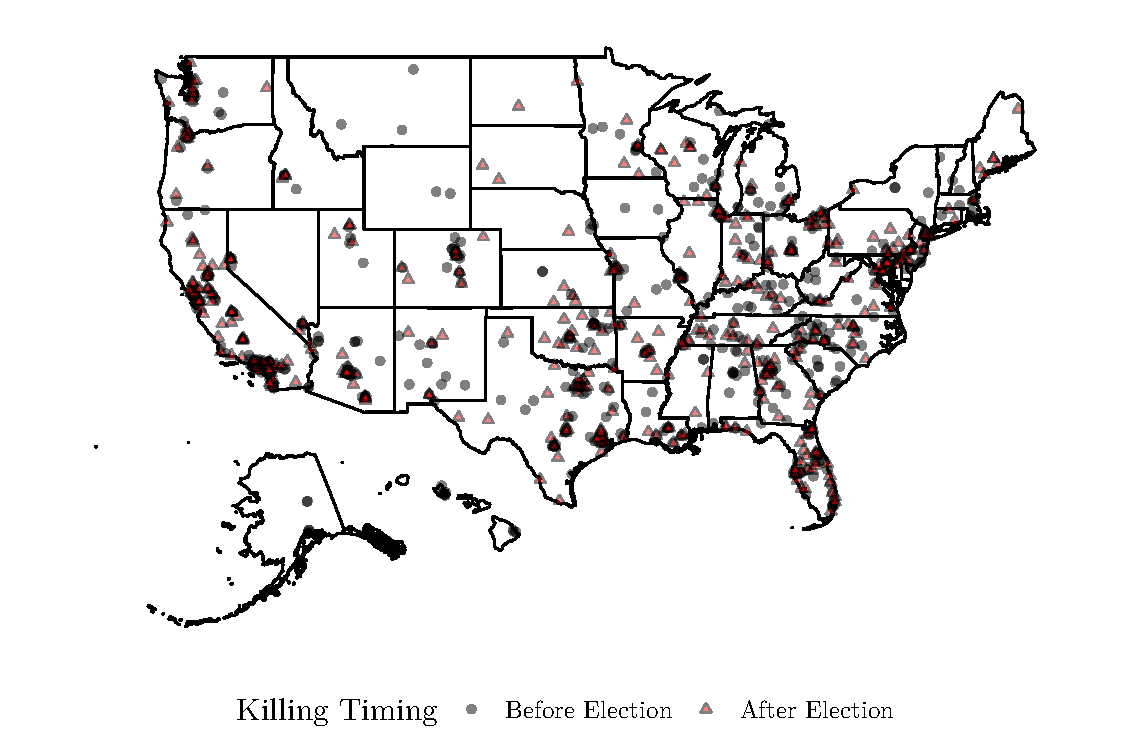
\includegraphics{shoot_to_files/figure-latex/map-16-1} 

}

\caption{\label{fig:map}Police Killing within 2 Months of Election, 2016 and 2020}\label{fig:map-16}
\end{figure}

\begin{figure}[h]

{\centering 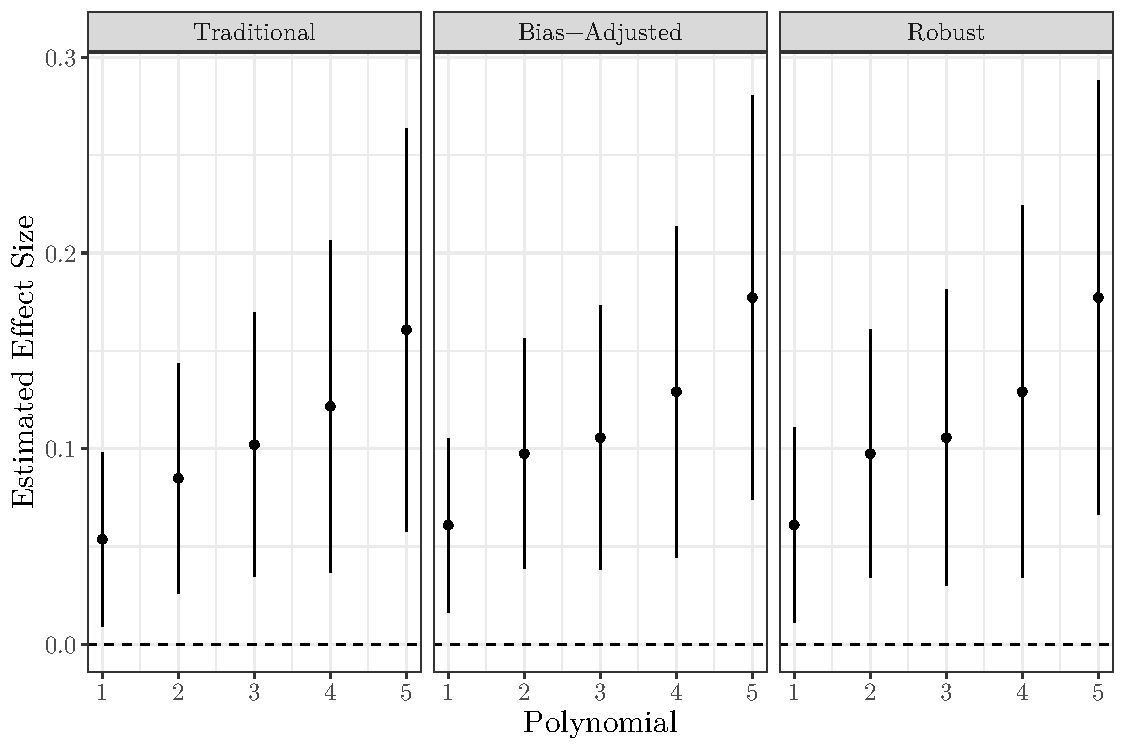
\includegraphics{shoot_to_files/figure-latex/diff-poly-1} 

}

\caption{\label{fig:map}Police Killing within 2 Months of Election, 2016 and 2020}\label{fig:diff-poly}
\end{figure}

\begin{figure}[h]

{\centering 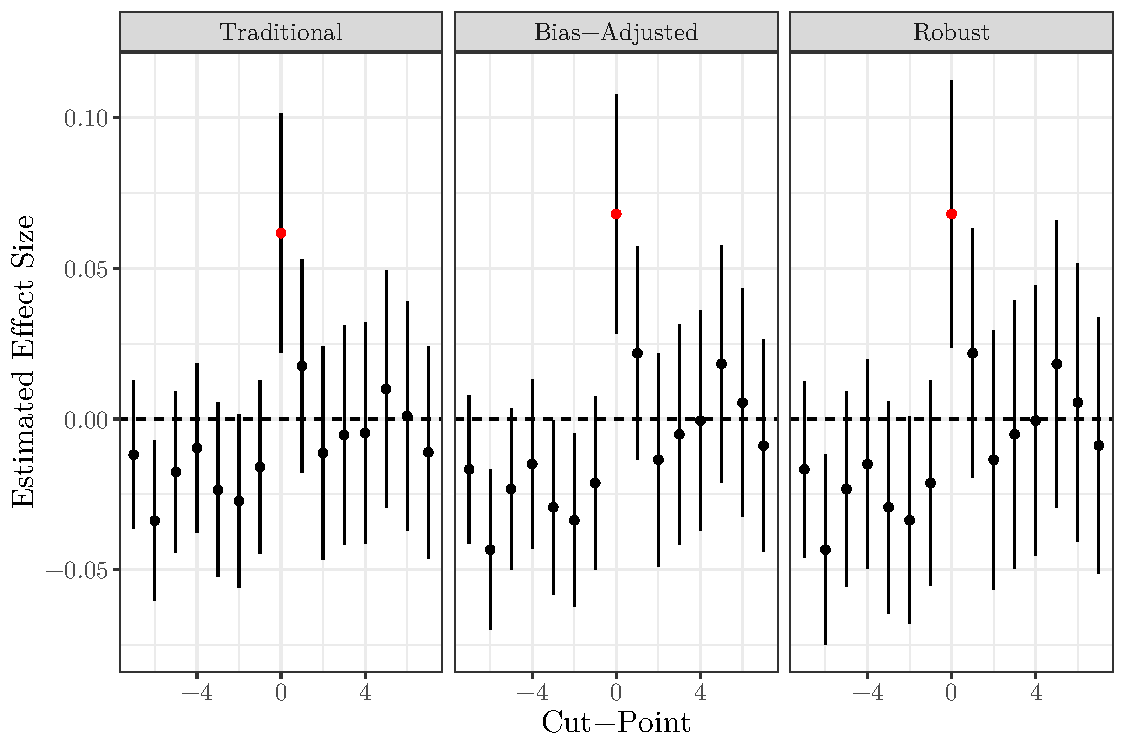
\includegraphics{shoot_to_files/figure-latex/placebo-cuts-1} 

}

\caption{\label{fig:map}Police Killing within 2 Months of Election, 2016 and 2020}\label{fig:placebo-cuts}
\end{figure}

\begin{figure}[h]

{\centering 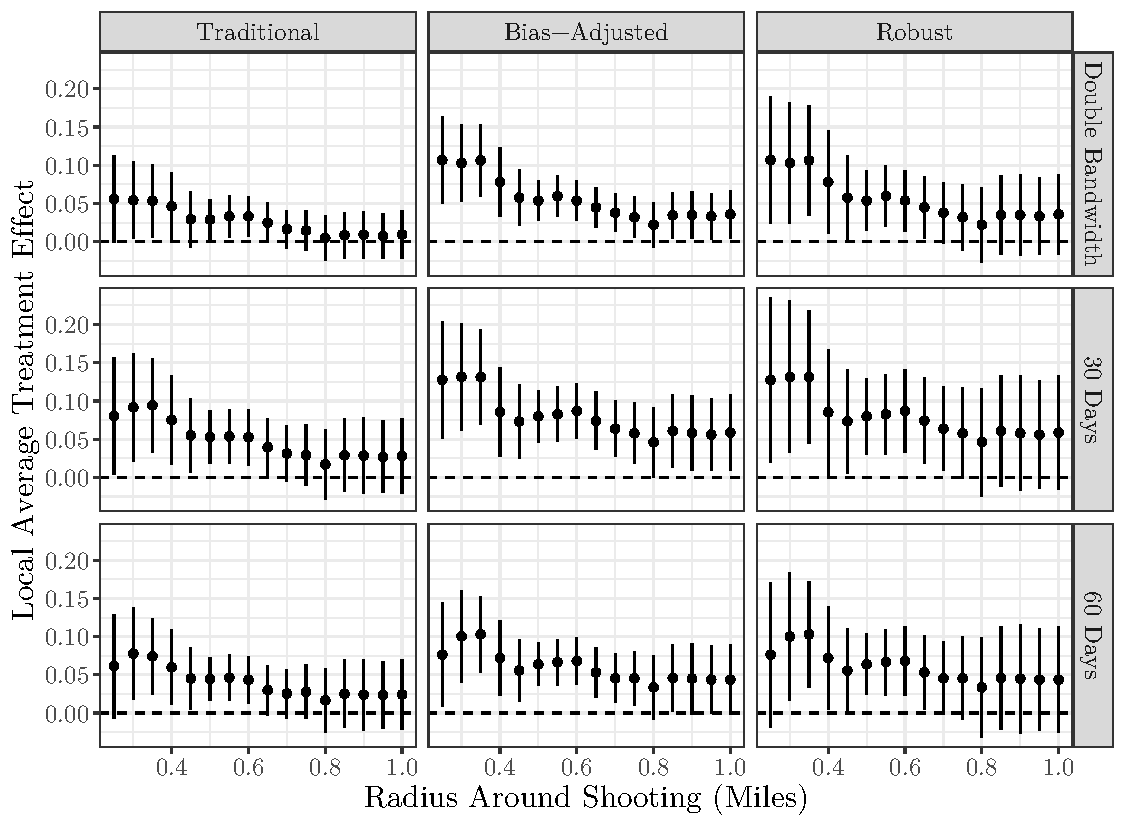
\includegraphics{shoot_to_files/figure-latex/bws-1} 

}

\caption{\label{fig:map}Police Killing within 2 Months of Election, 2016 and 2020}\label{fig:bws}
\end{figure}

\begin{figure}[h]

{\centering 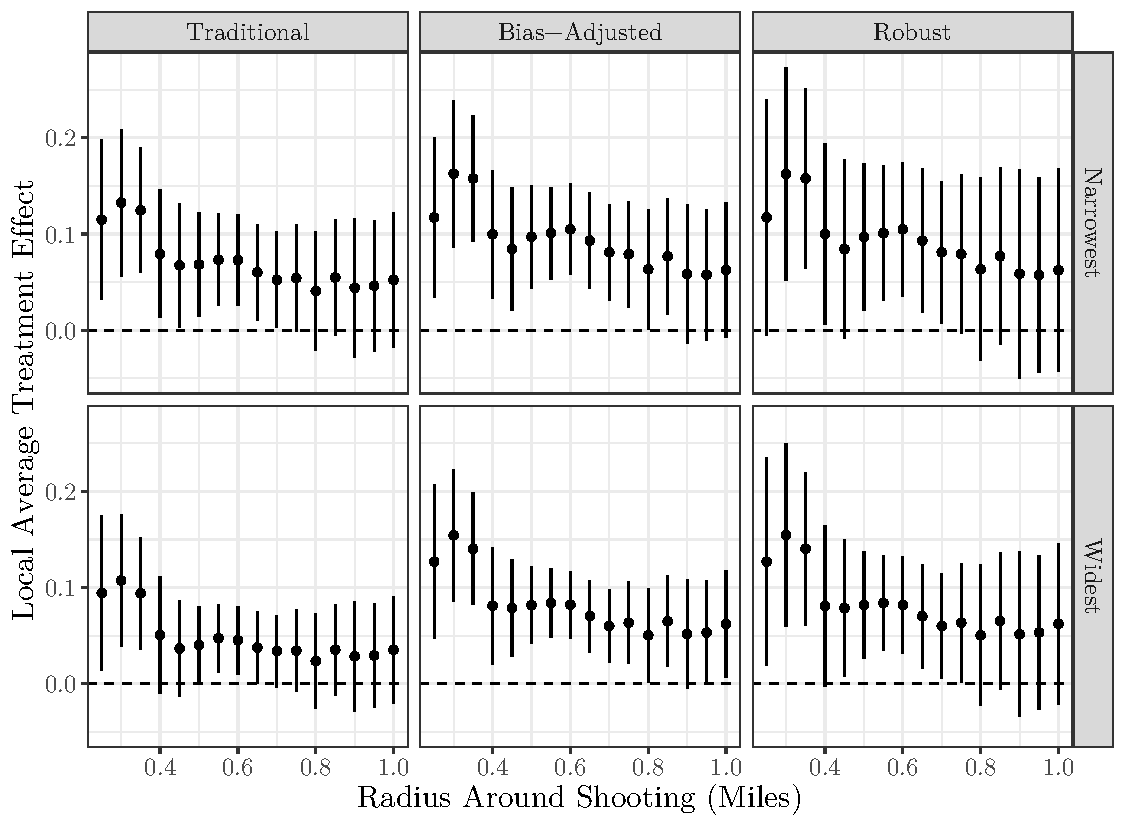
\includegraphics{shoot_to_files/figure-latex/bws-2-1} 

}

\caption{\label{fig:map}Police Killing within 2 Months of Election, 2016 and 2020}\label{fig:bws-2}
\end{figure}

\begin{figure}[h]

{\centering 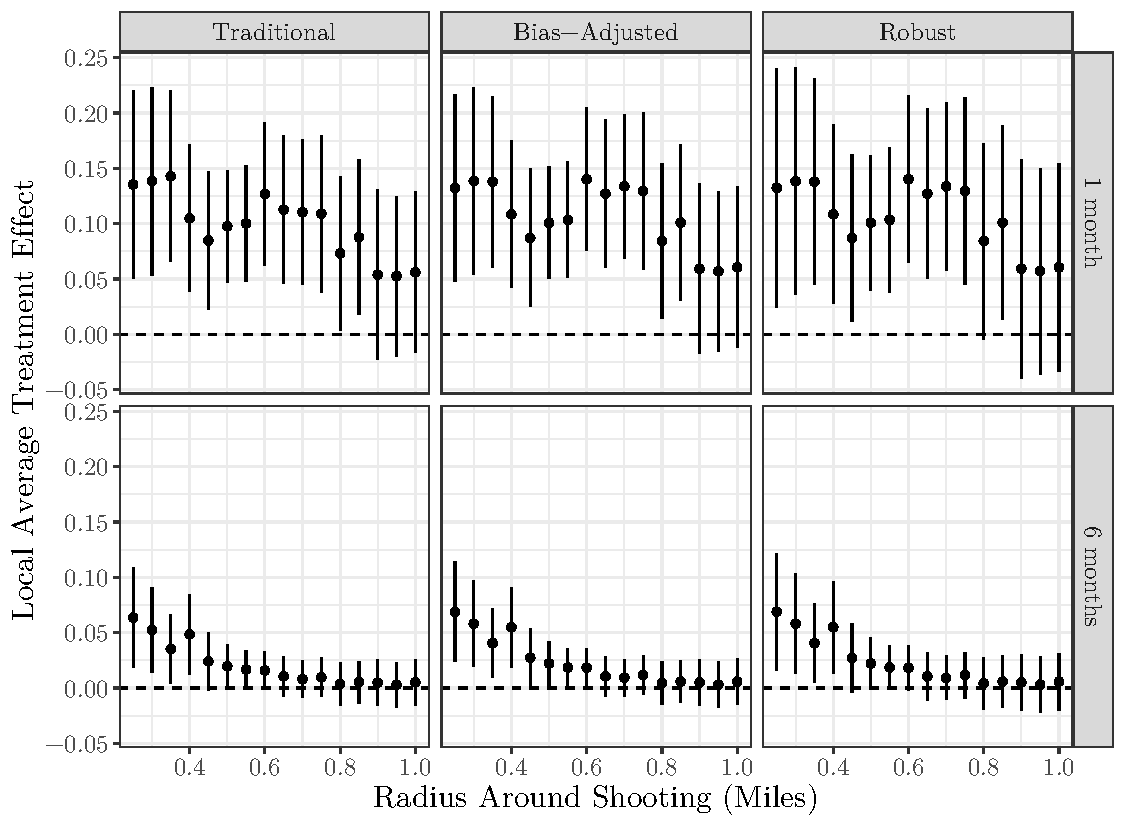
\includegraphics{shoot_to_files/figure-latex/bws-4-1} 

}

\caption{\label{fig:map}Police Killing within 2 Months of Election, 2016 and 2020}\label{fig:bws-4}
\end{figure}

\begin{figure}[h]

{\centering 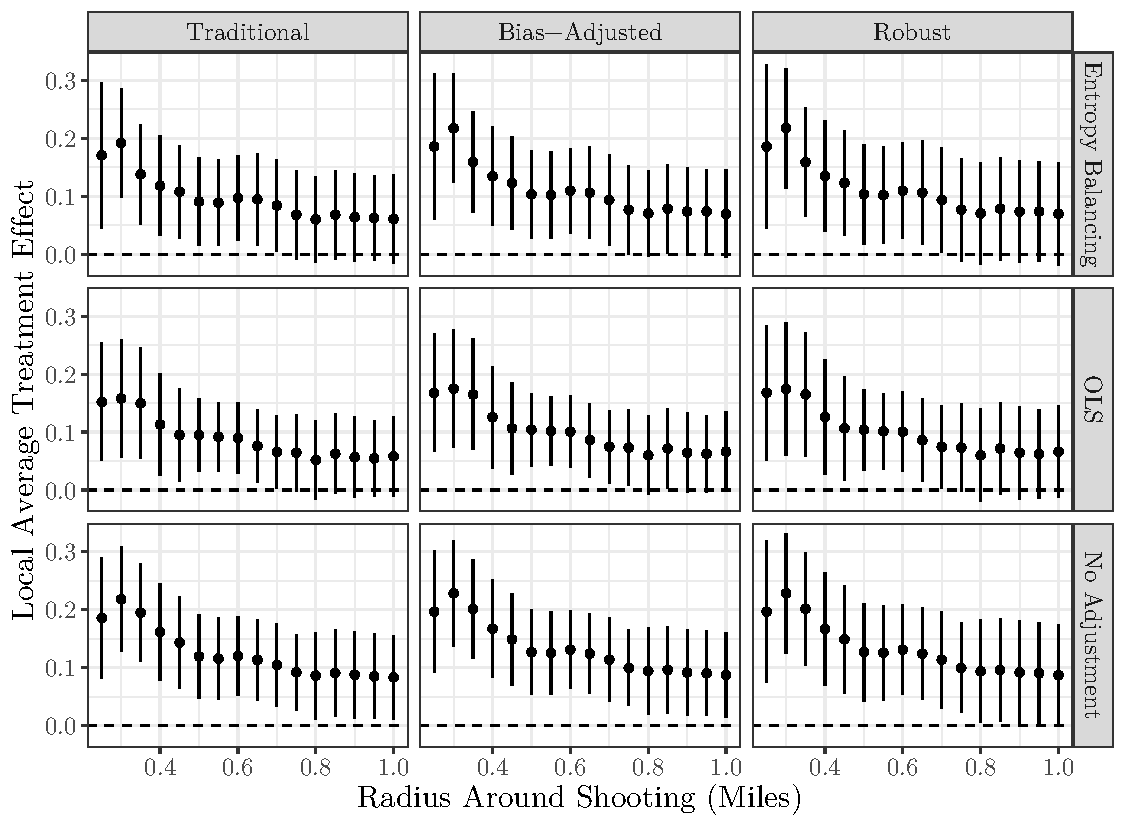
\includegraphics{shoot_to_files/figure-latex/alt-proc-1} 

}

\caption{\label{fig:map}Police Killing within 2 Months of Election, 2016 and 2020}\label{fig:alt-proc}
\end{figure}

\begin{figure}[h]

{\centering 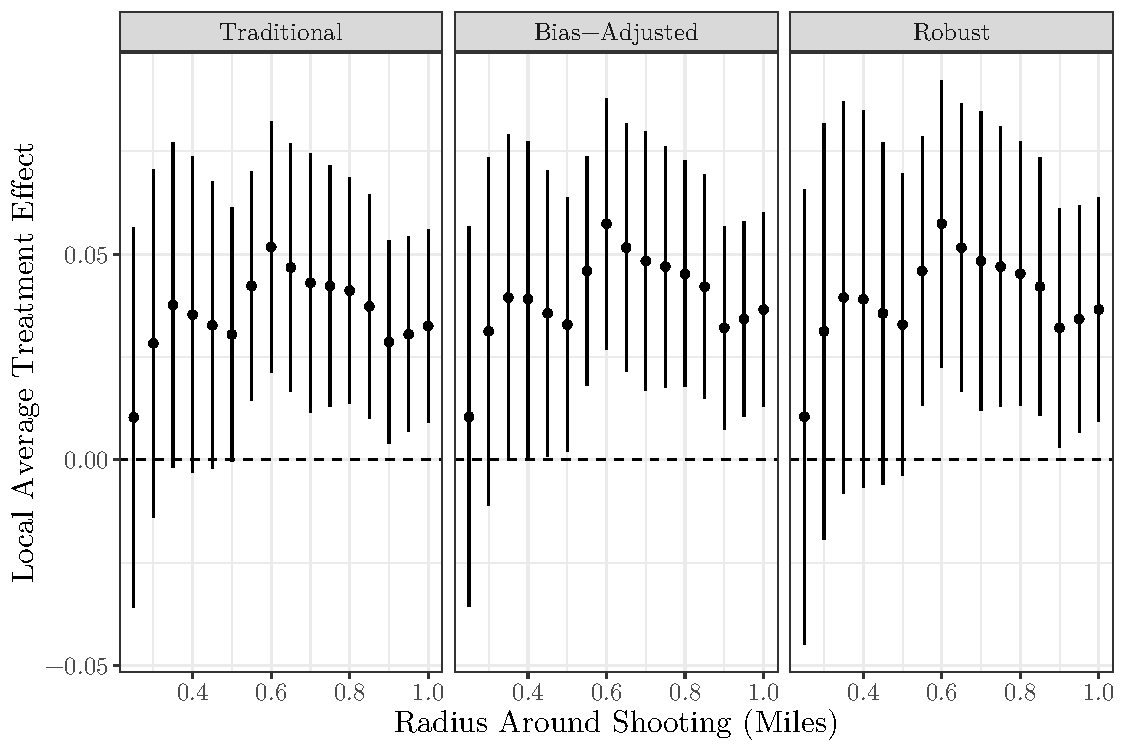
\includegraphics{shoot_to_files/figure-latex/placebo-prior-1} 

}

\caption{\label{fig:map}Police Killing within 2 Months of Election, 2016 and 2020}\label{fig:placebo-prior}
\end{figure}

\begin{figure}[h]

{\centering 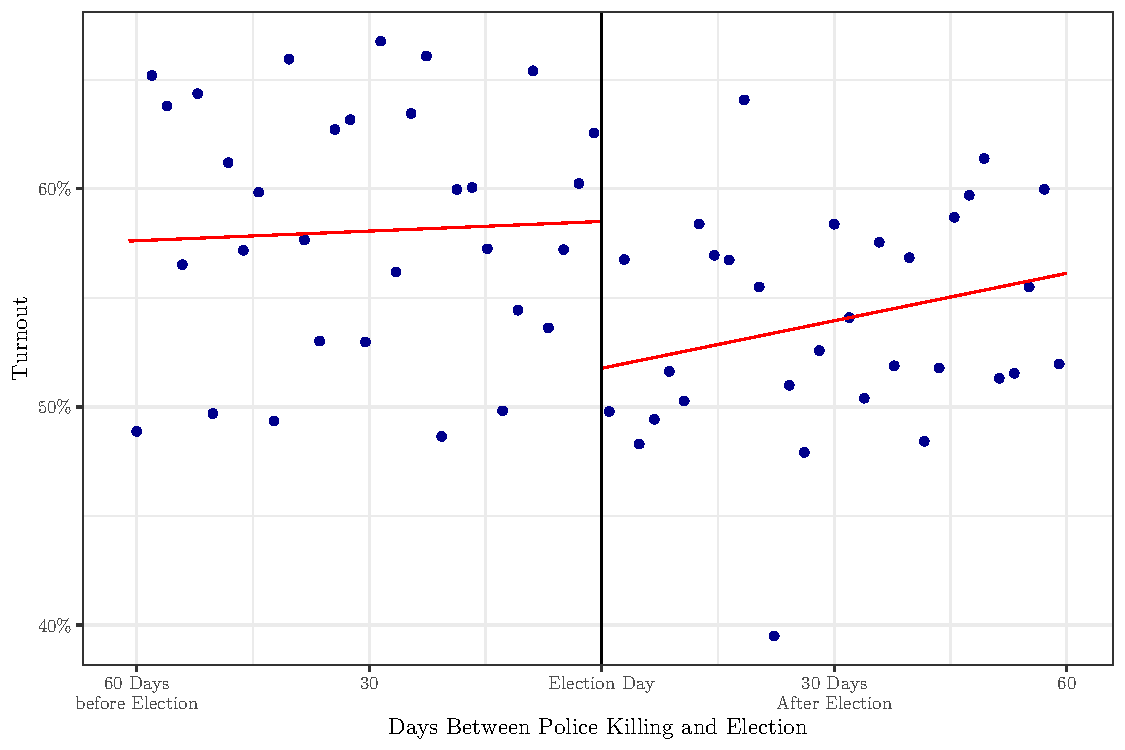
\includegraphics{shoot_to_files/figure-latex/rd-plot-1} 

}

\caption{\label{fig:map}Police Killing within 2 Months of Election, 2016 and 2020}\label{fig:rd-plot}
\end{figure}

\begin{figure}[h]

{\centering 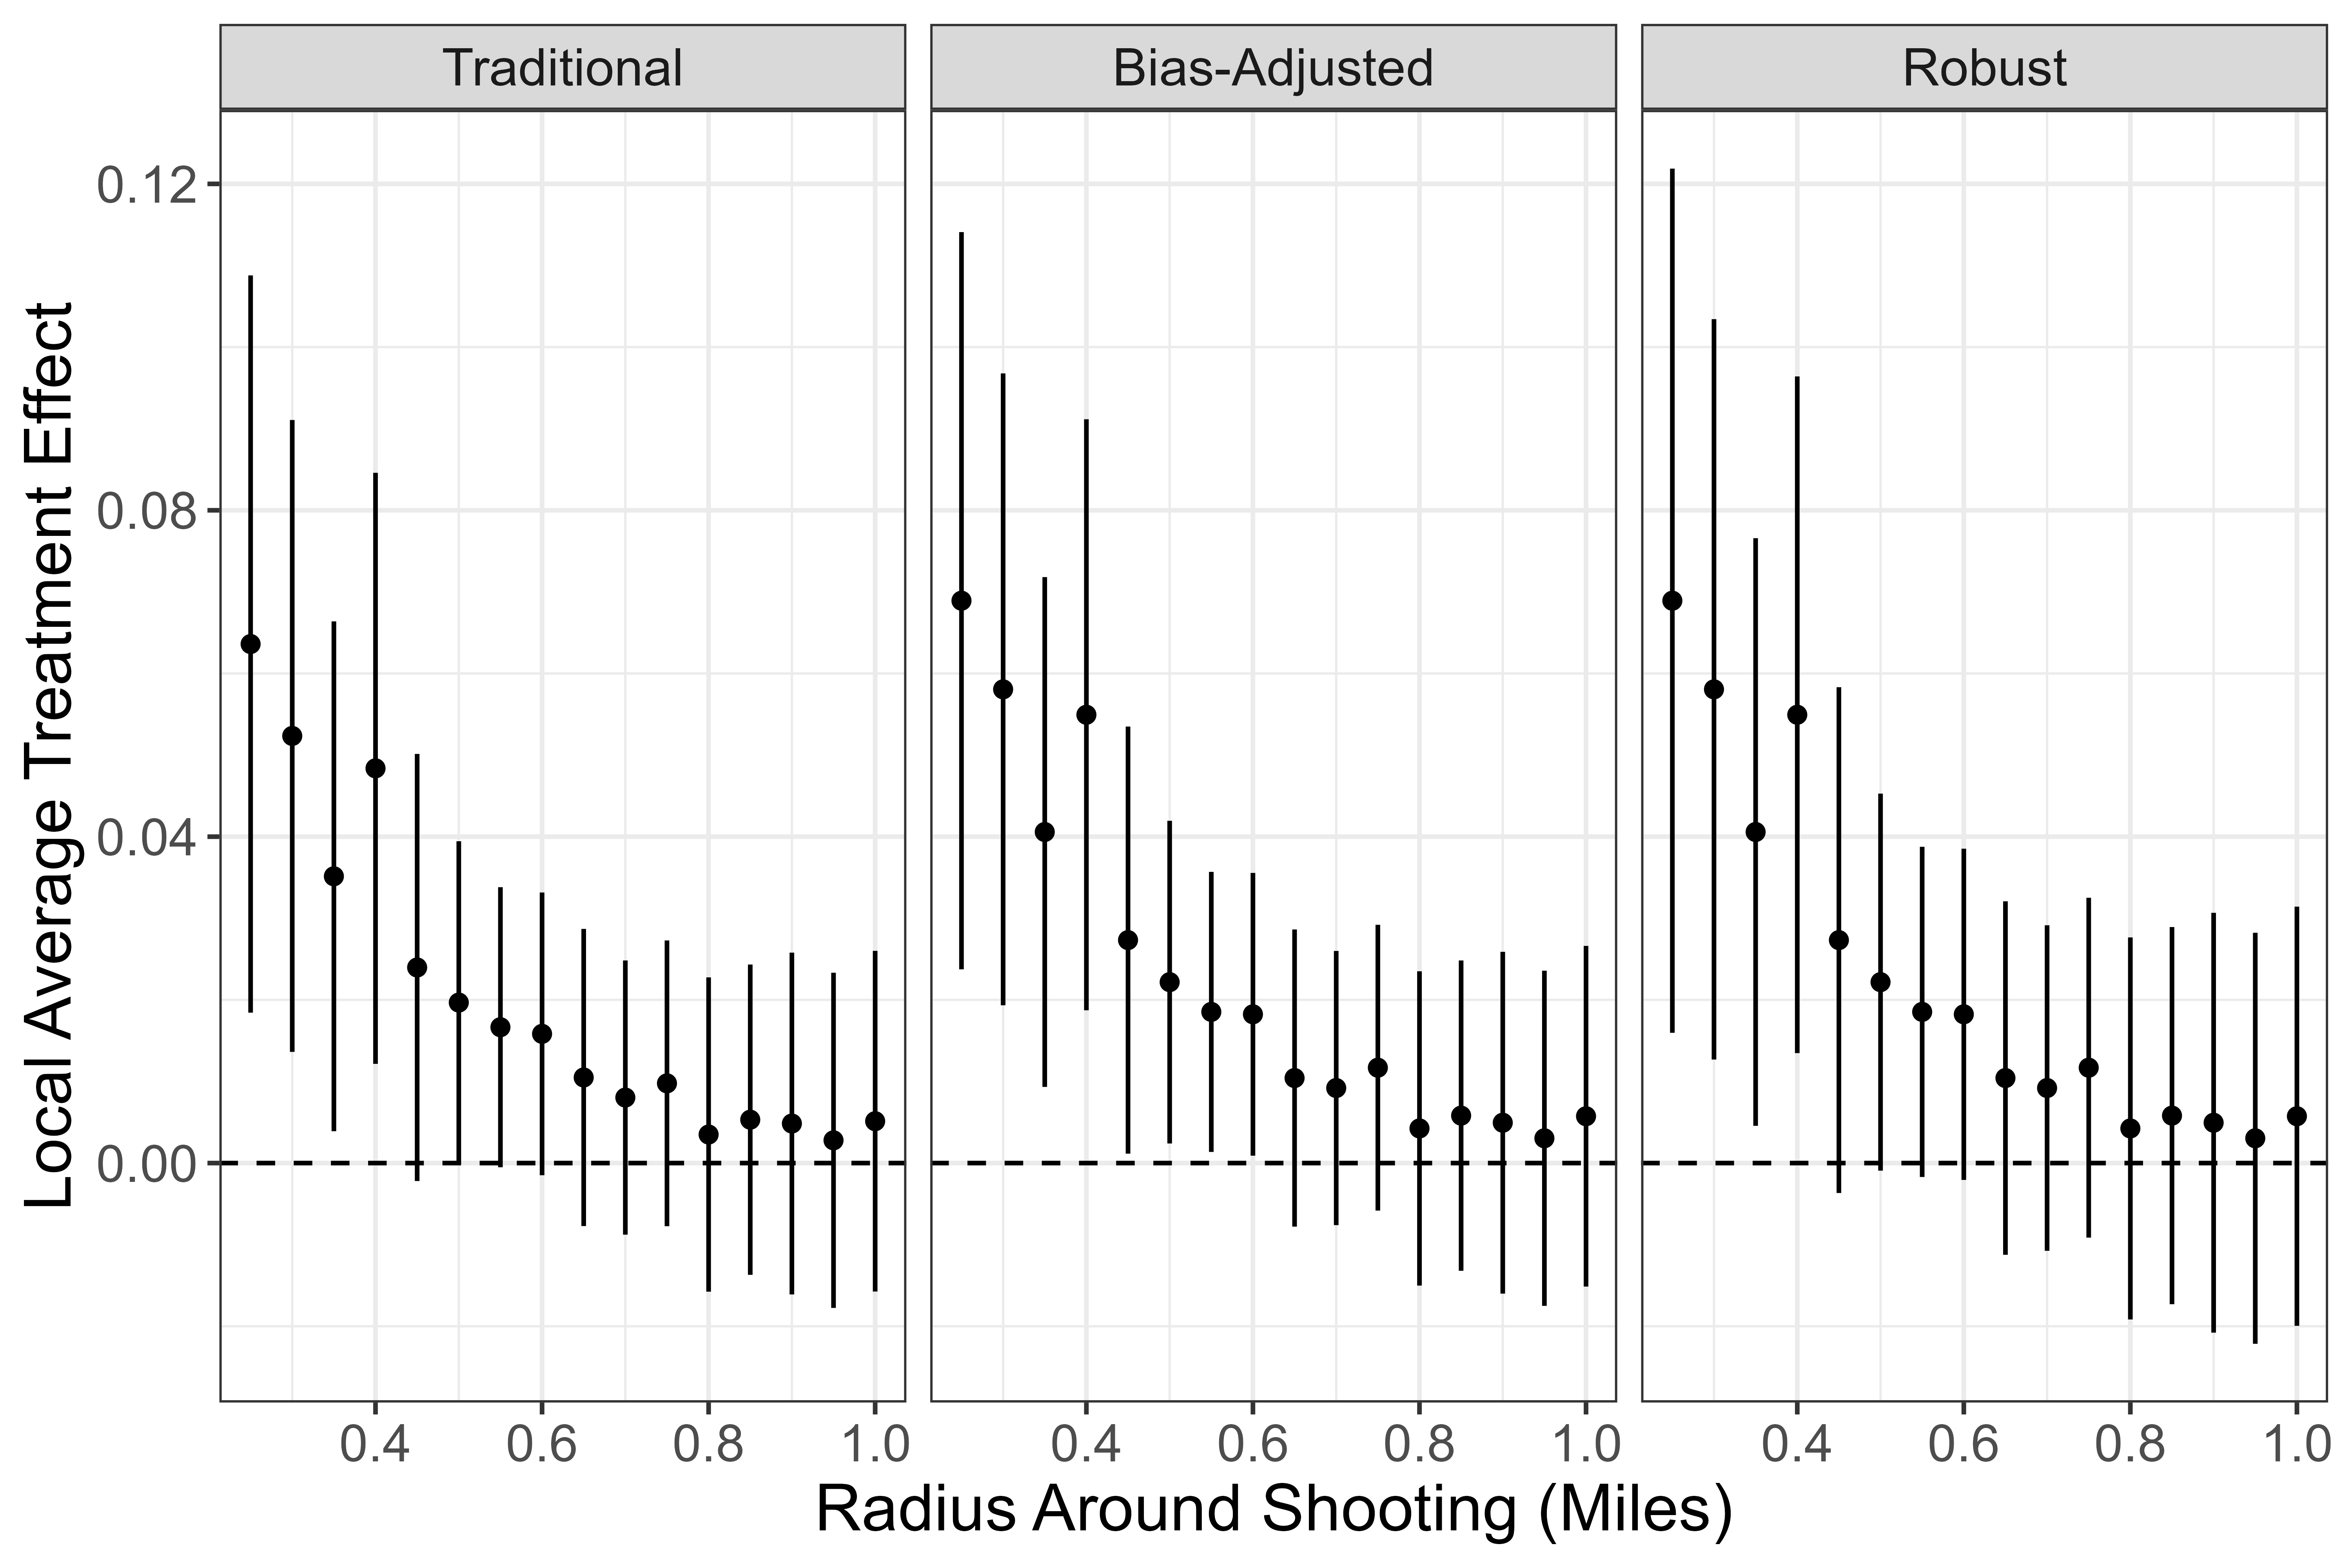
\includegraphics{shoot_to_files/figure-latex/dists-1} 

}

\caption{\label{fig:map}Police Killing within 2 Months of Election, 2016 and 2020}\label{fig:dists}
\end{figure}

\begin{figure}[h]

{\centering 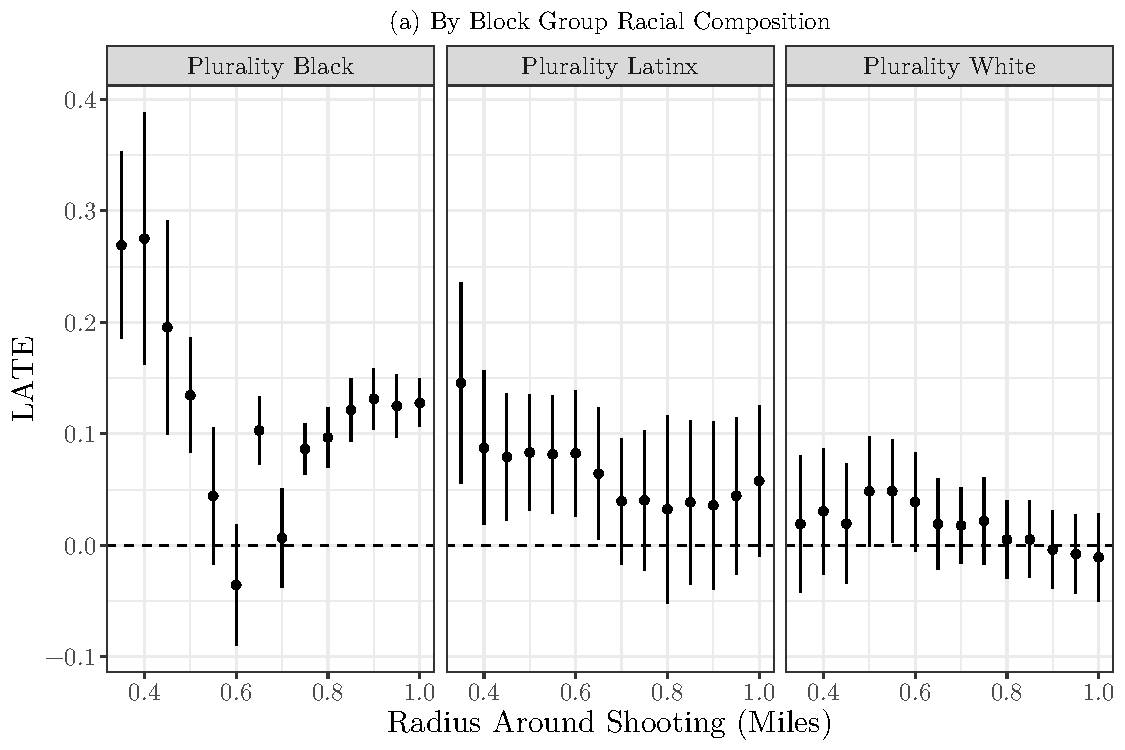
\includegraphics{shoot_to_files/figure-latex/nhood-1} 

}

\caption{\label{fig:map}Police Killing within 2 Months of Election, 2016 and 2020}\label{fig:nhood}
\end{figure}

\begin{figure}[h]

{\centering 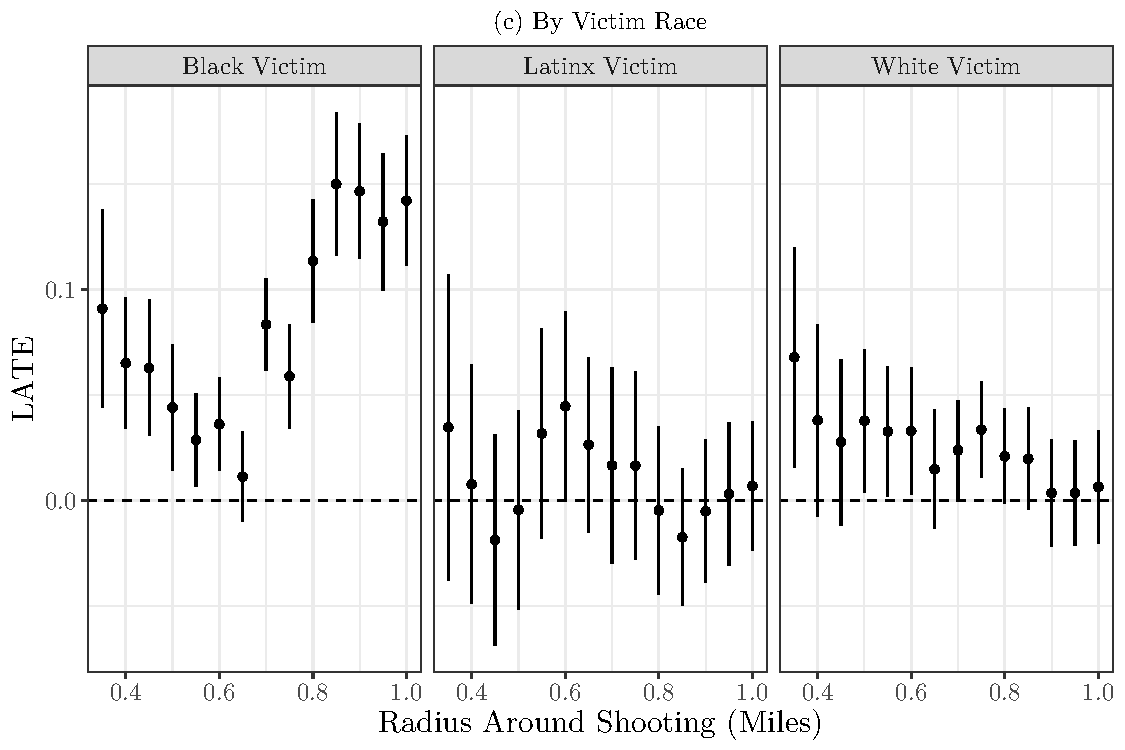
\includegraphics{shoot_to_files/figure-latex/victim-1} 

}

\caption{\label{fig:map}Police Killing within 2 Months of Election, 2016 and 2020}\label{fig:victim}
\end{figure}

\begin{figure}[h]

{\centering 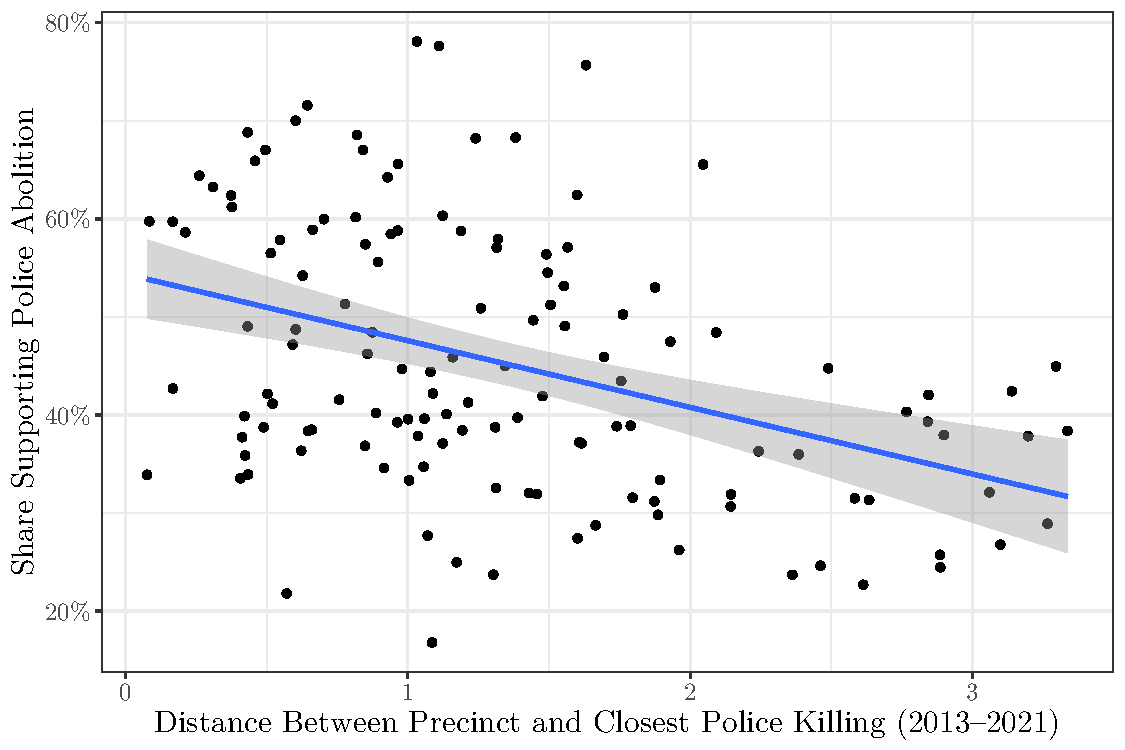
\includegraphics{shoot_to_files/figure-latex/minn-scatter-1} 

}

\caption{\label{fig:map}Police Killing within 2 Months of Election, 2016 and 2020}\label{fig:minn-scatter}
\end{figure}

\begin{figure}[h]

{\centering 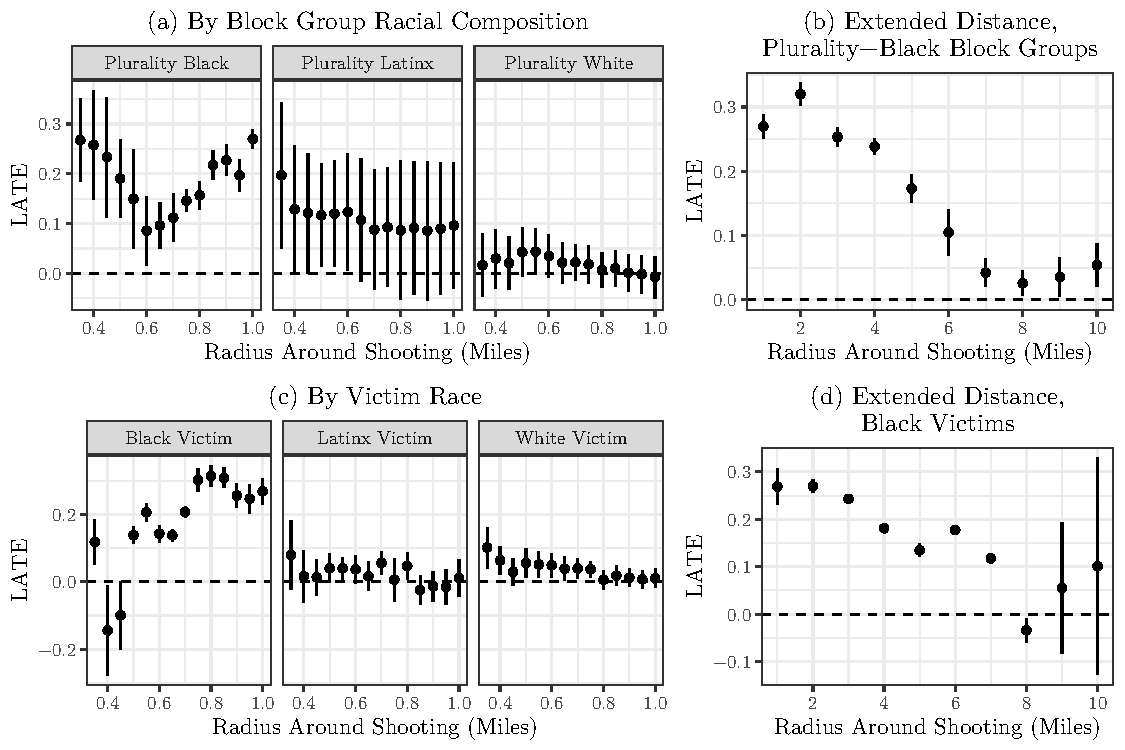
\includegraphics{shoot_to_files/figure-latex/paneled-race-effects-1} 

}

\caption{\label{fig:map}Police Killing within 2 Months of Election, 2016 and 2020}\label{fig:paneled-race-effects}
\end{figure}

\begin{figure}[h]

{\centering 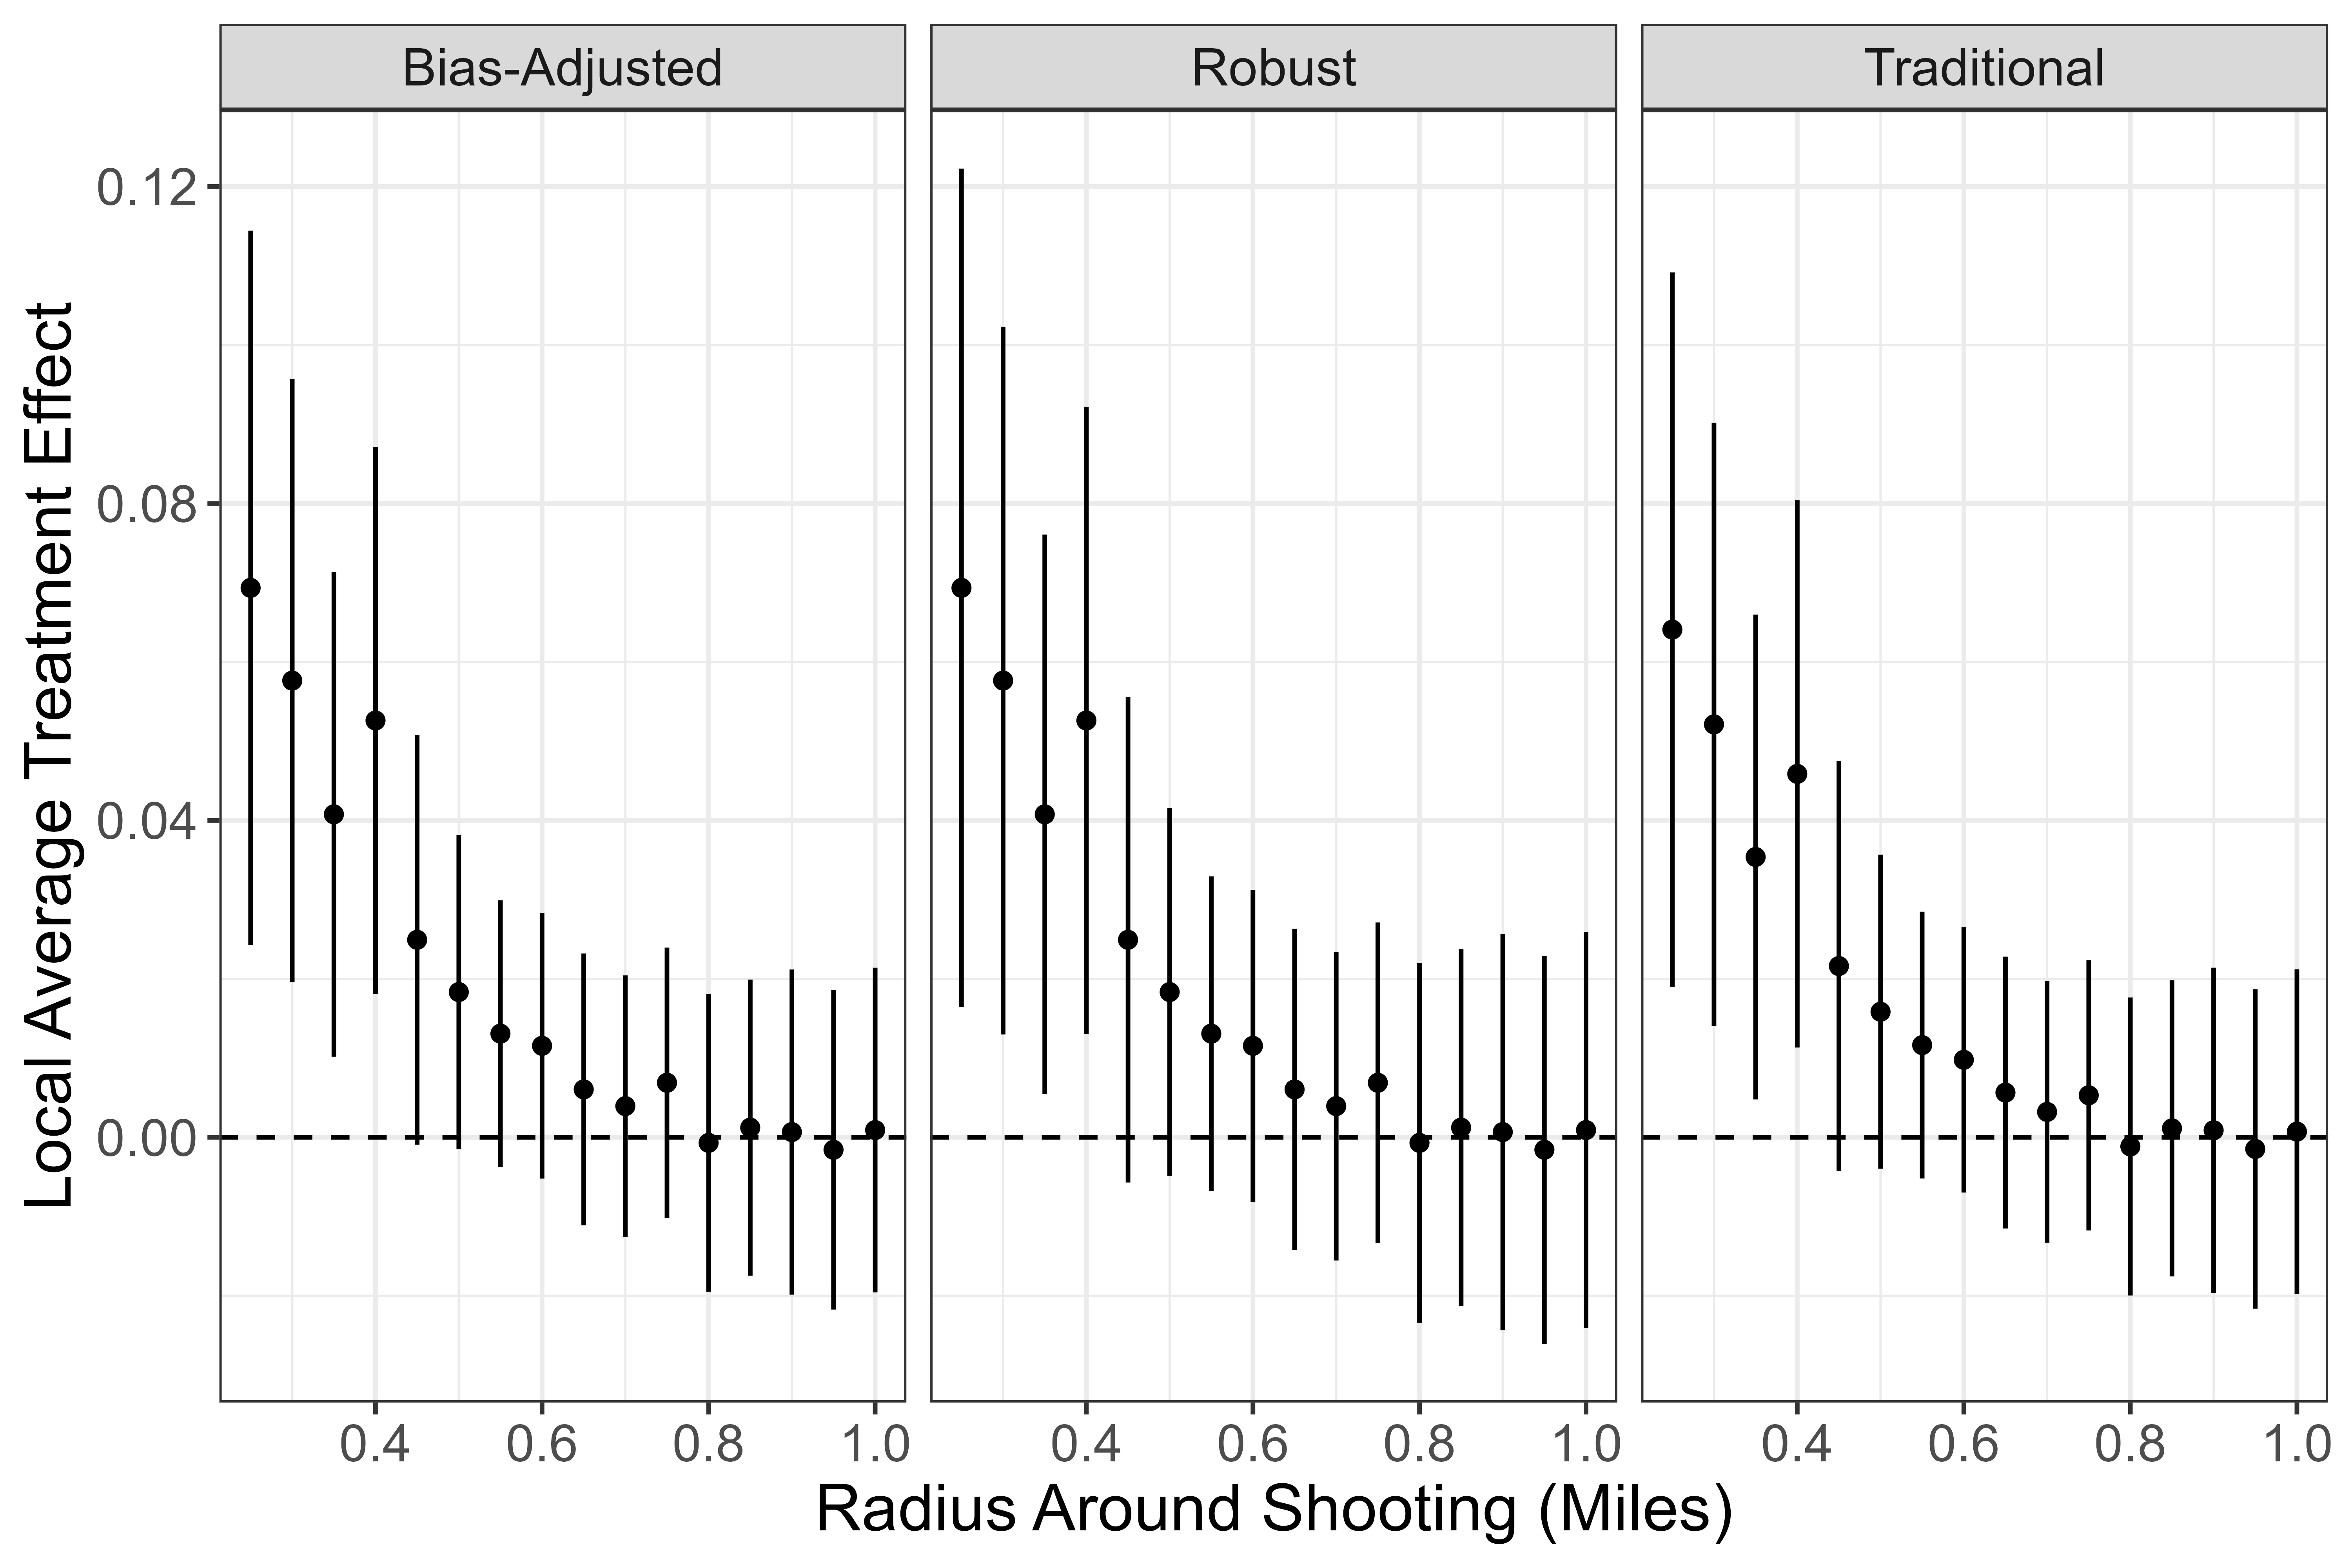
\includegraphics{shoot_to_files/figure-latex/first-difference-1} 

}

\caption{\label{fig:map}Police Killing within 2 Months of Election, 2016 and 2020}\label{fig:first-difference}
\end{figure}

\begin{figure}[h]

{\centering 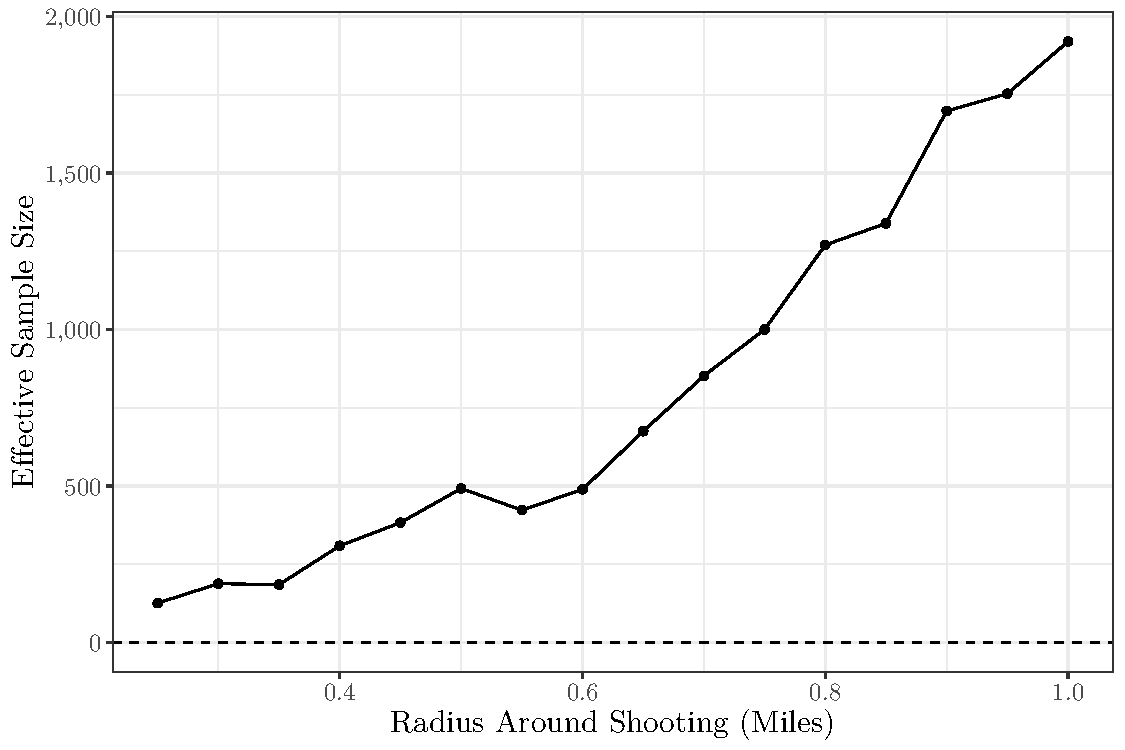
\includegraphics{shoot_to_files/figure-latex/samples-1} 

}

\caption{\label{fig:map}Police Killing within 2 Months of Election, 2016 and 2020}\label{fig:samples}
\end{figure}

\begin{figure}[h]

{\centering 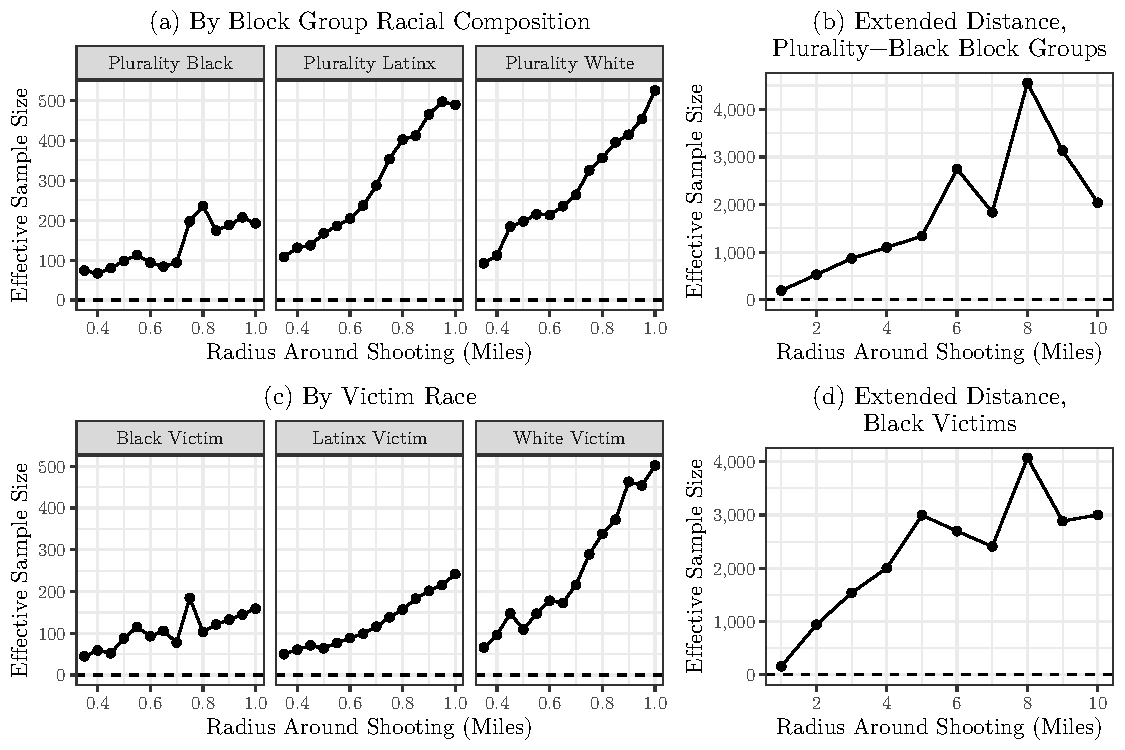
\includegraphics{shoot_to_files/figure-latex/samples-bo-1} 

}

\caption{\label{fig:map}Police Killing within 2 Months of Election, 2016 and 2020}\label{fig:samples-bo}
\end{figure}

\begin{figure}[h]

{\centering 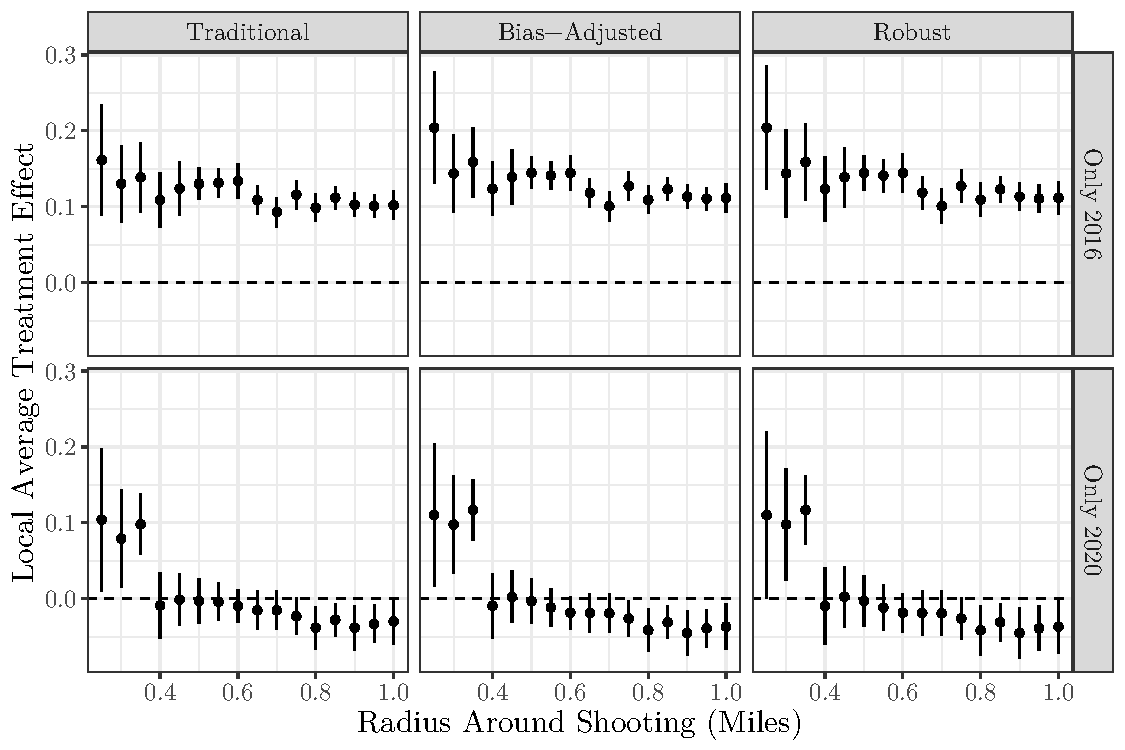
\includegraphics{shoot_to_files/figure-latex/individ-years-1} 

}

\caption{\label{fig:map}Police Killing within 2 Months of Election, 2016 and 2020}\label{fig:individ-years}
\end{figure}

\begin{singlespace}

 
\begin{table}[H]

\caption{\label{tab:balance-tab-full}\label{tab:full-bal} Demographics of Block Groups with Police Killings}
\centering
\begin{tabular}[t]{l>{\raggedright\arraybackslash}p{1in}>{\raggedright\arraybackslash}p{1in}>{\raggedright\arraybackslash}p{1in}>{\raggedright\arraybackslash}p{1in}}
\toprule
 & Not in Dataset & Treated & Unweighted Controls & Weighted Controls\\
\midrule
\addlinespace[0.3em]
\multicolumn{5}{l}{\textbf{2016}}\\
\hspace{1em}\% White & 64.2\% & 38.9\% & 31.3\% & 38.9\%\\
\hspace{1em}\% Black & 12.7\% & 20.4\% & 32.5\% & 20.4\%\\
\hspace{1em}\% Latino & 15.5\% & 29.2\% & 29.0\% & 29.2\%\\
\hspace{1em}\% Asian & 4.5\% & 8.0\% & 4.3\% & 8.0\%\\
\hspace{1em}Median Age & 40 & 36.4 & 34.6 & 36.4\\
\hspace{1em}\% with Some College & 57.9\% & 53.6\% & 49.0\% & 53.6\%\\
\hspace{1em}Median Income & \$60,877 & \$51,894 & \$43,365 & \$51,894\\
\hspace{1em}Population Density & 6,224 & 15,735 & 19,533 & 15,735\\
\hspace{1em}Previous Turnout & 35.9\% & 28.7\% & 26.4\% & 28.7\%\\
\hspace{1em}Number of Block Groups & 209,676 & 352 & 456 & 456\\
\hspace{1em}Number of Killings & 0 & 100 & 112 & 112\\
\addlinespace[0.3em]
\multicolumn{5}{l}{\textbf{2020}}\\
\hspace{1em}\% White & 62.5\% & 36.3\% & 30.7\% & 36.3\%\\
\hspace{1em}\% Black & 12.5\% & 17.2\% & 30.9\% & 17.2\%\\
\hspace{1em}\% Latino & 16.3\% & 39.0\% & 28.5\% & 39.0\%\\
\hspace{1em}\% Asian & 4.9\% & 3.8\% & 5.9\% & 3.8\%\\
\hspace{1em}Median Age & 40.9 & 36.4 & 37 & 36.4\\
\hspace{1em}\% with Some College & 60.1\% & 50.6\% & 53.2\% & 50.6\%\\
\hspace{1em}Median Income & \$72,351 & \$56,413 & \$61,800 & \$56,413\\
\hspace{1em}Population Density & 6,636 & 26,215 & 29,386 & 26,215\\
\hspace{1em}Previous Turnout & 49.6\% & 44.2\% & 40.2\% & 44.2\%\\
\hspace{1em}Number of Block Groups & 158,653 & 391 & 338 & 338\\
\hspace{1em}Number of Killings & 0 & 113 & 103 & 103\\
\bottomrule
\end{tabular}
\end{table}
 
\end{singlespace}

\end{document}
